\chapter{Moti di punti materiali e vincoli.}
\section{Moto di un punto materiale}
\begin{center}
    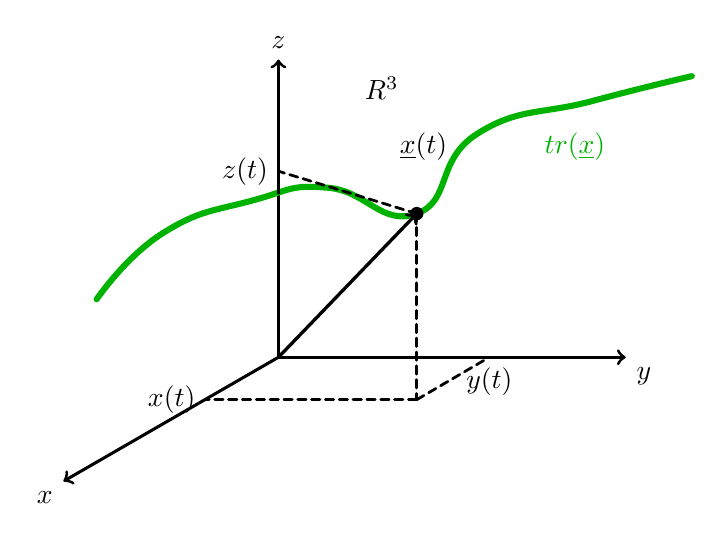
\begin{tikzpicture}[scale=1.05, line cap=round, line join=round]

% --- assi in "prospettiva" (2D) ---
\coordinate (O) at (0,0);
\coordinate (X) at (-2.6,-1.5);
\coordinate (Y) at (4.2,0);
\coordinate (Z) at (0,3.6);

\draw[->,line width=1.1pt] (O) -- (X) node[below left] {$x$};
\draw[->,line width=1.1pt] (O) -- (Y) node[below right] {$y$};
\draw[->,line width=1.1pt] (O) -- (Z) node[above] {$z$};

% --- base per le coordinate in 2D ---
\coordinate (Xhat) at (-0.65,-0.38);
\coordinate (Yhat) at (1,0);
\coordinate (Zhat) at (0,1);

% punto P = a*Xhat + b*Yhat + c*Zhat
\def\xa{1.35}
\def\yb{2.55}
\def\zc{2.25}
\coordinate (P) at ({\xa*(-0.65)+\yb},{\xa*(-0.38)+\zc});

% proiezioni
\coordinate (Px) at ({\xa*(-0.65)},{\xa*(-0.38)});
\coordinate (Py) at (\yb,0);
\coordinate (Pz) at (0,\zc);
\coordinate (Pxy) at ({\xa*(-0.65)+\yb},{\xa*(-0.38)});
\node[black,anchor=west] at (\xa , \yb) {$\underline{x}(t)$};

% --- traiettoria verde (passa ESATTAMENTE per P) ---
\draw[green!70!black,line width=2.2pt]
  plot[smooth,tension=0.85]
  coordinates {(-2.2,0.7) (-1.4,1.5) (-0.3,1.9) (0.6,2.05) (P) (2.4,2.7) (3.8,3.1) (5.0,3.4)};
\node[green!70!black,anchor=west] at (3.1,2.55) { $\operatorname{tr}(\underline{x})$};

% --- vettore posizione ---
\draw[->,line width=1.2pt] (O) -- (P);

% --- punto ---
\fill (P) circle (2.3pt);

% --- proiezioni tratteggiate ---
\draw[densely dashed,line width=1.0pt] (P) -- (Pxy);
\draw[densely dashed,line width=1.0pt] (Pxy) -- (Py) node[below] {$y(t)$};
\draw[densely dashed,line width=1.0pt] (Pxy) -- (Px) node[left] {$x(t)$};
\draw[densely dashed,line width=1.0pt] (P) -- (Pz) node[left] {$z(t)$};
\draw[densely dashed,line width=1.0pt] (Pz) -- (O);

% etichette extra
\node at (1.25,3.25) {$\mathbb{R}^3$};


\end{tikzpicture}
\end{center}
Possiamo modellare il moto di un punto materiale tramite una legge oraria del tipo
\[
\underline{x}(t) = (x(t) , y(t) , z(t))
\]
Matematicamente stiamo descrivendo una curva parametrizzata in $\mathbb{R}^3$ del tipo $\underline{x}:[0 , t_f] \to \mathbb{R}^3$.
\begin{oss}{}
La stessa traccia (traiettoria) può essere percorsa con diverse leggi orarie $\underline{x}(t)$ che matematicamente corrispondono a diverse riparametrizzazioni equivalenti di una curva.
\end{oss}
Possiamo quindi definire la velocità della curva come il vettore tangente alla curva dato da
\[
 \underline{v}(t)= \underline{\dot{x}}(t) =\frac{d\underline{x}}{dt}
=\left(\frac{dx}{dt},\,\frac{dy}{dt},\,\frac{dz}{dt}\right)
\]
e il vettore accelerazione dato da
\[
\frac{d^2\underline{x}}{dt^2}=\underline{a}
=\frac{d\underline{v}}{dt}
=(a_x,a_y,a_z).
\]

\begin{center}
\begin{tikzpicture}[scale=1.05, line cap=round, line join=round]

% --- assi in "prospettiva" (2D) ---
\coordinate (O) at (0,0);
\draw[->,line width=1.1pt] (O) -- (-2.4,-1.4);
\draw[->,line width=1.1pt] (O) -- (5.0,0);
\draw[->,line width=1.1pt] (O) -- (0,3.6);

% --- punto sulla curva ---
\coordinate (P) at (3.0,2.65);
\fill (P) circle (2.4pt);

% --- curva (passa per P) ---
\draw[line width=2.0pt]
  plot[smooth,tension=0.9]
  coordinates {(-3.0,1.0) (-1.5,2.2) (0.8,2.9) (P) (4.0,2.25) (5.2,2.55) (6.0,3.0)};

% --- vettore velocità (tangente) ---
\draw[->,line width=1.15pt] (P) -- ++(1.7,-0.25)
  node[below right] {$\underline{v}$};

% --- accelerazione totale (ancora più piccola) ---
\coordinate (Aend) at ($(P)+(0.55,-0.69)$); % più corta
\draw[->,line width=1.15pt] (P) -- (Aend)
  node[below right] {$\underline{a}$};

% --- componenti: a parallela e a perpendicolare (somma = a) ---
\coordinate (Apar)  at ($(P)+(0.63,-0.09)$);
\coordinate (Aperp) at ($(P)+(-0.08,-0.60)$);

\draw[->,line width=1.05pt] (P) -- (Apar)
  node[above right] {$\underline{a}_{\parallel}$};

\draw[->,line width=1.05pt] (P) -- (Aperp)
  node[left] {$\underline{a}_{\perp}$};

\end{tikzpicture}
\end{center}

Possiamo descrivere un moto in coordinate diverse dalle coordinate cartesiane.\\
Se il moto è nel piano ($z=0$) allora una scelta di coordinate può essere quella delle coordinate polari.
\begin{center}
\begin{tikzpicture}[scale=1.1, line cap=round, line join=round]

% assi
\draw[->,line width=1.1pt] (-0.8,0) -- (5.2,0);
\draw[->,line width=1.1pt] (0,-0.8) -- (0,3.6);

% punto finale
\coordinate (P) at (4,2.8);
\fill (P) circle (2.3pt);

% vettore r
\draw[line width=1.2pt] (0,0) -- (P);
\node[ right] at ($(0,0)!0.72!(P)$) {$\rho$};

% proiezioni tratteggiate
\draw[densely dashed,line width=1.0pt] (P) -- (4,0);
\draw[densely dashed,line width=1.0pt] (P) -- (0,2.8);

% etichette assi vicino alle proiezioni
\node[below] at (4,0) {$x$};
\node[left]  at (0,2.8) {$y$};

% angolo theta
\draw[line width=1.0pt] (1,0) arc[start angle=0,end angle=35,radius=1];
\node at (1.25,0.35) {$\theta$};

\end{tikzpicture}
\end{center}

Le coordinate polari sono date da
\[
(\rho(x(t) , y(t)) , \theta(x(t) , y(t))) = (\sqrt{x^2 +y^2} , \operatorname{arctg}(y/x))
\]
o equivalentemente da
\[
\underline{x}(t) = (x(\theta(t) , \rho(t)) ,y(\theta(t) , \rho(t))) = (\rho \cos\theta  , \rho\sin\theta)
\]
Possiamo anche riscrivere $\underline{v}(t)$ attraverso le coordinate polari.
\[
v_x=\frac{dx}{dt}
=\frac{d}{dt}\bigl(\rho\cos\theta\bigr)
=\frac{d\rho}{dt}\cos\theta-\rho\sin\theta\,\frac{d\theta}{dt}
=\dot{\rho}\cos\theta-\rho\sin\theta\,\dot{\theta}.
\]

\[
v_y=\frac{dy}{dt}
=\frac{d}{dt}\bigl(\rho\sin\theta\bigr)
=\dot{\rho}\sin\theta+\rho\dot{\theta}\cos\theta.
\]

\[
\underline{v}=(v_x,v_y)
=
\dot{\rho}
\begin{pmatrix}
\cos\theta\\
\sin\theta
\end{pmatrix}
+
\rho\dot{\theta}
\begin{pmatrix}
-\sin\theta\\
\cos\theta
\end{pmatrix} = \dot{\rho} \cdot \underline{e_\rho} + \rho \dot{\theta} \cdot \underline{e_\theta} , \quad \underline{e_\rho}\cdot \underline{e_\theta}=0
\]

\begin{center}
\begin{tikzpicture}[scale=1.05, line cap=round, line join=round]

% assi
\draw[->,line width=1.2pt] (-3.2,0) -- (5.2,0) node[below right] {$x$};
\draw[->,line width=1.2pt] (0,-3.0) -- (0,3.6) node[above] {$y$};

% circonferenza tratteggiata
\pgfmathsetmacro{\R}{2.6}
\draw[dashed, line width=1.1pt] (0,0) circle (\R);

% punto P sulla circonferenza a 45°
\pgfmathsetmacro{\Px}{\R/sqrt(2)}
\pgfmathsetmacro{\Py}{\R/sqrt(2)}
\coordinate (P) at (\Px,\Py);

% raggio tratteggiato
\draw[dashed, line width=1.1pt] (0,0) -- (P);

% punto
\fill (P) circle (2.4pt);

% --- curva nera: due Bézier che si incontrano in P con tangente verticale ---
% scegli due punti finali della curva (a sinistra-alto e a destra-basso)
\coordinate (A) at (1.5,3.25);
\coordinate (B) at (5.3,0.95);

% controlli: quelli vicini a P sono verticali (stesso x = Px) => tangente verticale in P
\coordinate (c1) at (2.2,3.15);            % controllo vicino ad A
\coordinate (c2) at (\Px,\Py+1.25);        % controllo sopra P (verticale)
\coordinate (c3) at (\Px,\Py-1.15);        % controllo sotto P (verticale)
\coordinate (c4) at (4.4,0.55);            % controllo vicino a B

\draw[line width=3.0pt]
  (A) .. controls (c1) and (c2) .. (P)
      .. controls (c3) and (c4) .. (B);

% --- vettori in P ---
% v: tangente alla curva in P (verticale)
\draw[->,green!70!black,line width=2.0pt] (P) -- ++(0,1.15)
  node[above] {$\underline{v}$};

% t: tangente alla circonferenza in P (direzione (-1,1))
\draw[->,red!75!black,line width=2.0pt] (P) -- ++(-0.75,0.75)
  node[above left] {$\underline{e_\theta}$};

% m: radiale (perpendicolare alla circonferenza) in P (direzione (1,1))
\draw[->,red!75!black,line width=2.0pt] (P) -- ++(0.75,0.75)
  node[above right] {$\underline{e_\rho}$};
% angolo \theta (archetto all'origine tra asse x e raggio OP)
\draw[line width=1.0pt] (0.9,0) arc[start angle=0,end angle=45,radius=0.9];
\node at (0.75,0.25) {$\theta$};

% lunghezza \rho sul raggio (etichetta lungo il segmento OP)
\node at ($(0,0)!0.55!(P)$) {$\rho$};
\end{tikzpicture}
\end{center}
\begin{oss}{}
    Il versore $\underline{e_\theta}$ non è tangente alla curva ma alla circonferenza centrata nell'origine di raggio $\rho$ nel punto $\underline{x}(t)$. Di conseguenza non è tangente alla velocità.
\end{oss}
Ricaviamo infine il vettore accelerazione $\underline{a}(t)$ in coordinate polari.
\[
a_x=\frac{dv_x}{dt}
=\frac{d}{dt}\bigl(\dot{\rho}\cos\theta-\rho\,\dot{\theta}\sin\theta\bigr)
=\ddot{\rho}\cos\theta-\dot{\rho}\dot{\theta}\sin\theta-\dot{\rho}\dot{\theta}\sin\theta
-\rho\,\frac{d}{dt}\bigl(\dot{\theta}\sin\theta\bigr)
\]
\[
=\ddot{\rho}\cos\theta-2\dot{\rho}\dot{\theta}\sin\theta
-\rho\Bigl(\ddot{\theta}\sin\theta+(\dot{\theta})^2\cos\theta\Bigr)
\]
\[
=\ddot{\rho}\cos\theta-2\dot{\rho}\dot{\theta}\sin\theta-\rho\,\ddot{\theta}\sin\theta-\rho(\dot{\theta})^2\cos\theta
\]
\[
=\bigl(\ddot{\rho}-\rho(\dot{\theta})^2\bigr)\cos\theta-\bigl(2\dot{\rho}\dot{\theta}+\rho\ddot{\theta}\bigr)\sin\theta.
\]

\[
a_y=\frac{d}{dt}v_y
=\frac{d}{dt}\bigl(\dot{\rho}\sin\theta+\rho\,\dot{\theta}\cos\theta\bigr)
=\ddot{\rho}\sin\theta+\dot{\rho}\dot{\theta}\cos\theta+\dot{\rho}\dot{\theta}\cos\theta
+\rho\,\frac{d}{dt}\bigl(\dot{\theta}\cos\theta\bigr)
\]
\[
=\ddot{\rho}\sin\theta+2\dot{\rho}\dot{\theta}\cos\theta
+\rho\Bigl(\ddot{\theta}\cos\theta-(\dot{\theta})^2\sin\theta\Bigr)
\]
\[
=\ddot{\rho}\sin\theta+2\dot{\rho}\dot{\theta}\cos\theta+\rho\,\ddot{\theta}\cos\theta-\rho(\dot{\theta})^2\sin\theta
\]
\[
=\bigl(\ddot{\rho}-\rho(\dot{\theta})^2\bigr)\sin\theta+\bigl(\rho\ddot{\theta}+2\dot{\rho}\dot{\theta}\bigr)\cos\theta.
\]

\[
\Rightarrow\quad
\underline{a}=(a_x,a_y)
=\bigl(\ddot{\rho}-\rho\dot{\theta}^{\,2}\bigr)\,
\underbrace{\begin{pmatrix}\cos\theta\\ \sin\theta\end{pmatrix}}_{\underline{e}_{\rho}}
+\bigl(\rho\ddot{\theta}+2\dot{\rho}\dot{\theta}\bigr)\,
\underbrace{\begin{pmatrix}-\sin\theta\\ \cos\theta\end{pmatrix}}_{\underline{e}_{\theta}}.
\]

Per un generico moto (e quindi per una generica traiettoria) le coordinate polari non hanno un reale vantaggio, anzi complicano di parecchio le cose. Possono però essere utili per descrivere specifici moti ad esempio il moto circolare di raggio costante $R$.

\begin{itemize}
\item Con le coordinate cartesiane devo avere 2 informazioni per definire
$\underline{x}(t)$, $\underline{v}(t)$, $\underline{a}(t)$.

\item Se uso le coordinate polari $\rho=R$ definisco il moto fornendo solamente un'informazione ovvero $\theta(t)$.
\end{itemize}
\begin{center}
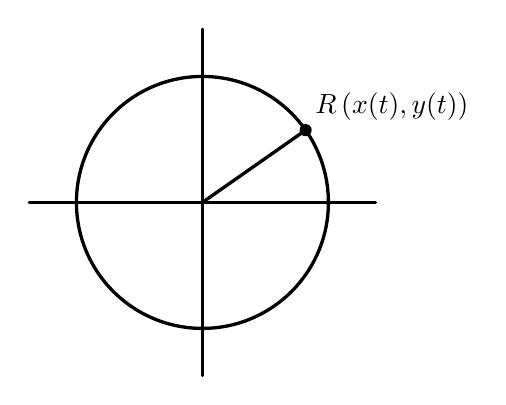
\begin{tikzpicture}[scale=1.0, line cap=round, line join=round]
  \def\R{1.6}
  \def\ang{35}

  % assi
  \draw[line width=1.1pt] (-2.2,0) -- (2.2,0);
  \draw[line width=1.1pt] (0,-2.2) -- (0,2.2);

  % cerchio
  \draw[line width=1.2pt] (0,0) circle (\R);

  % punto e raggio
  \coordinate (P) at ({\R*cos(\ang)},{\R*sin(\ang)});
  \draw[line width=1.2pt] (0,0) -- (P);
  \fill (P) circle (2.2pt);

  % etichetta R(x(t),y(t))
  \node[above right] at (P) {$R\,(x(t),y(t))$};
\end{tikzpicture}
\end{center}
La velocità infatti diventa
\[
\underline{v}=\rho\,\dot{\theta}
\begin{pmatrix}
-\sin\theta\\
\cos\theta
\end{pmatrix}
=R\dot{\theta}\,\underline{t}.
\]
\begin{center}
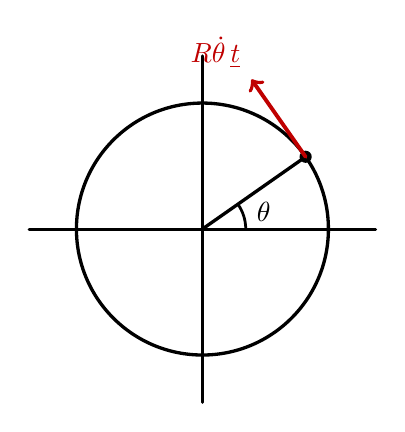
\begin{tikzpicture}[scale=1.0, line cap=round, line join=round]
  \def\R{1.6}
  \def\ang{35}

  % assi
  \draw[line width=1.1pt] (-2.2,0) -- (2.2,0);
  \draw[line width=1.1pt] (0,-2.2) -- (0,2.2);

  % cerchio
  \draw[line width=1.2pt] (0,0) circle (\R);

  % punto e raggio
  \coordinate (P) at ({\R*cos(\ang)},{\R*sin(\ang)});
  \draw[line width=1.2pt] (0,0) -- (P);
  \fill (P) circle (2.2pt);

  % angolo theta
  \draw[line width=1.0pt] (0.55,0) arc[start angle=0,end angle=\ang,radius=0.55];
  \node at (0.78,0.22) {$\theta$};

  % velocità: R dot(theta) t
  \draw[->,red!75!black,line width=1.4pt]
    (P) -- ++({-1.2*sin(\ang)},{1.2*cos(\ang)})
    node[above left] {$R\dot{\theta}\,\underline{t}$};
\end{tikzpicture}
\end{center}
mentre l'accelerazione diventa
\[
\underline{a}
=-R\dot{\theta}^{\,2}
\begin{pmatrix}
\cos\theta\\
\sin\theta
\end{pmatrix}
+R\ddot{\theta}
\begin{pmatrix}
-\sin\theta\\
\cos\theta
\end{pmatrix}
=
-R\dot{\theta}^{\,2}\,\underline{n}+R\ddot{\theta}\,\underline{t}.
\]

\begin{center}
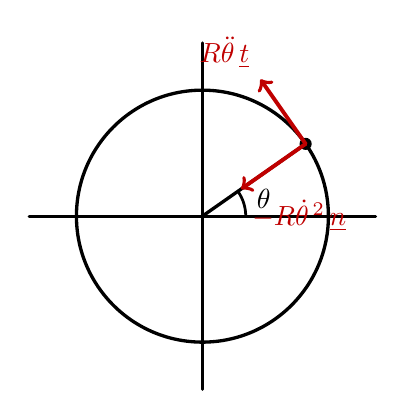
\begin{tikzpicture}[scale=1.0, line cap=round, line join=round]
  \def\R{1.6}
  \def\ang{35}

  % assi
  \draw[line width=1.1pt] (-2.2,0) -- (2.2,0);
  \draw[line width=1.1pt] (0,-2.2) -- (0,2.2);

  % cerchio
  \draw[line width=1.2pt] (0,0) circle (\R);

  % punto e raggio
  \coordinate (P) at ({\R*cos(\ang)},{\R*sin(\ang)});
  \draw[line width=1.2pt] (0,0) -- (P);
  \fill (P) circle (2.2pt);

  % angolo theta
  \draw[line width=1.0pt] (0.55,0) arc[start angle=0,end angle=\ang,radius=0.55];
  \node at (0.78,0.22) {$\theta$};

  % componente tangenziale: R ddot(theta) t
  \draw[->,red!75!black,line width=1.4pt]
    (P) -- ++({-1.0*sin(\ang)},{1.0*cos(\ang)})
    node[above left] {$R\ddot{\theta}\,\underline{t}$};

  % componente normale: -R dot(theta)^2 m (verso il centro)
  \draw[->,red!75!black,line width=1.4pt]
    (P) -- ++({-1.0*cos(\ang)},{-1.0*sin(\ang)})
    node[below right] {$-R\dot{\theta}^{\,2}\,\underline{n}$};
\end{tikzpicture}
\end{center}
\begin{oss}{}
 $\ddot{\theta}(t)$ potrebbe essere negativo e quindi $R\ddot{\theta}\,\underline{t}$ potrebbe avere direzione $-\underline{t}$.
\end{oss}

\begin{oss}{}
    In questo caso i versori $\underline{e_\theta}, \underline{e_\rho}$ corrispondono (a meno del verso) con i versori $\underline{n} , \underline{t}$ normale e tangente alla curva.
\end{oss}

\section{Introduzione ai vincoli e loro classificazione}
Nel paragrafo precedente abbiamo introdotto la descrizione cinematica di un punto materiale. Consideriamo ora un insieme di $n$ punti materiali detto sistema di punti materiali. Ogni punto del sistema è descritto da una legge oraria
\[
\underline{x_i} (t) = (x_i(t) , y_i(t) , z_i(t)) \quad \forall i = 1 \ldots , n
\]
In generale, un sistema di $n$ punti  materiali non è completamente libero: i punti sono spesso soggetti a restrizioni geometriche o cinematiche, dette vincoli, che ne limitano i moti ammissibili legando tra loro le coordinate.\\
Queste condizioni e relazioni sul moto vengono dette $\textbf{vincoli}$.
\begin{example}{}
    Consideriamo un punto che si muove di moto piano. La sua traiettoria è descritta da una curva del tipo
    \[
    \underline{x}(t) = (x(t) , y(t) , z(t))
    \]
    e dal vincolo $z = 0$. Per descrivere il moto del punto sono quindi sufficienti 2 informazioni che in questo caso corrispondono a $(x(t) , y(t))$.
\end{example}

\begin{example}{}
    Possiamo rivedere l'esempio del moto circolare nell'ottica dei vincoli. Abbiamo 1 punto che si muove con traiettoria $(x(t) , y(t) , z(t))$ e 2 vincoli ovvero
    \[
    \begin{cases}
        z = 0 \\
        x^2 + y^2 = R^2
    \end{cases}
    \]
    Il sistema può essere descritto da una sola coordinata $\theta(t)$
\end{example}

\begin{example}{}
Consideriamo $2$ punti materiali nello spazio:
\[
\bigl(x_1(t),y_1(t),z_1(t)\bigr), \qquad \bigl(x_2(t),y_2(t),z_2(t)\bigr).
\]
In assenza di vincoli, per descrivere il sistema servono $6$ coordinate (tre per ciascun punto).

Supponiamo ora di imporre il vincolo che la distanza tra i due punti sia fissata e pari a $d$. Il vincolo si scrive come
\[
\bigl(x_1-x_2\bigr)^2+\bigl(y_1-y_2\bigr)^2+\bigl(z_1-z_2\bigr)^2=d^2.
\]
Il sistema può essere descritto da 5 coordinate.
\end{example}

\begin{example}{}
Consideriamo un punto materiale nello spazio:
\[
\bigl(x(t),y(t),z(t)\bigr).
\]
In assenza di vincoli, per descrivere il sistema servono $3$ coordinate.

Supponiamo ora che il punto sia vincolato a muoversi su una superficie sferica di raggio $R$. Il vincolo si scrive come
\[
x^2+y^2+z^2=R^2.
\]
Il sistema può essere descritto da 2 coordinate.
\end{example}

\begin{example}{}
Consideriamo il moto di due punti materiali sul piano con distanza fissata tra di loro:
\[
\bigl(x_1(t),y_1(t),z_1(t)\bigr),\qquad \bigl(x_2(t),y_2(t),z_2(t)\bigr).
\]
I vincoli sono
\[
z_1=0,\qquad z_2=0,\qquad (x_1-x_2)^2+(y_1-y_2)^2=d^2.
\]

Possiamo usare coordinate ``convenienti'': ad esempio scegliere come coordinate indipendenti
\[
(x_1(t),\,y_1(t),\,\theta(t)),
\]
dove $\theta(t)$ è l'angolo che il segmento che unisce i due punti forma con l'asse $x$ e dove $x_1 , y_1$ sono le coordinate nel piano del centro del segmento che li congiunge.

\medskip

\begin{center}
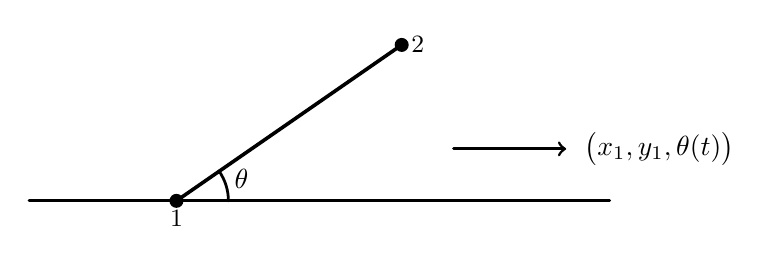
\begin{tikzpicture}[scale=1.1, line cap=round, line join=round]

% asse orizzontale
\draw[line width=1.1pt] (-0.5,0) -- (6.2,0);

% punti 1 e 2
\coordinate (P1) at (1.2,0);
\coordinate (P2) at (3.8,1.8);

\fill (P1) circle (2.3pt) node[below] {\small $1$};
\fill (P2) circle (2.3pt) node[right] {\small $2$};

% segmento tra i punti
\draw[line width=1.3pt] (P1) -- (P2);

% angolo theta in P1
\draw[line width=1.0pt] (1.8,0) arc[start angle=0,end angle=35,radius=0.6];
\node at (1.95,0.25) {$\theta$};

% freccia e testo (x1,y1,theta(t))
\draw[->,line width=1.0pt] (4.4,0.6) -- (5.7,0.6);
\node[anchor=west] at (5.8,0.6) {$\bigl(x_1,y_1,\theta(t)\bigr)$};

\end{tikzpicture}
\end{center}
\end{example}

Dopo aver visto alcuni esempi introduttivi presentiamo una classificazione dei vincoli.
\begin{itemize}
\item \textbf{Monolatero posizionale:}
\[
g(x_1,x_2,\dots,x_m,t)\ge 0.
\]

\item \textbf{Monolatero posizionale indipendente dal tempo:}
\[
g(x_1,x_2,\dots,x_m)\ge 0.
\]

\item \textbf{Bilatero posizionale:}
\[
g(x_1,\dots,x_m,t)=0.
\]

\item \textbf{Bilatero posizionale indipendente dal tempo:}
\[
g(x_1,\dots,x_m)=0.
\]
\end{itemize}

\begin{example}{}
(\textbf{Monolatero posizionale}) Un punto vincolato a rimanere nel semispazio superiore:
\[
z(t)\ge 0.
\]
\end{example}

\begin{example}{}
(\textbf{Bilatero posizionale, dipendente dal tempo}) Un punto vincolato a stare su una circonferenza di raggio $R(t)$, dove $R(t)$ è una legge nota:
\[
g\bigl((x(t),y(t)),t\bigr)=x^2(t)+y^2(t)-R^2(t)=0.
\]
\end{example}

\begin{example}{}
(\textbf{Monolatero posizionale, dipendente dal tempo}) Un punto vincolato a stare all'esterno (o sul bordo) della circonferenza di raggio $R(t)$:
\[
x^2(t)+y^2(t)-R^2(t)\ge 0.
\]
\end{example}

\begin{itemize}
\item \textbf{Vincoli dipendenti dalla velocità non integrabili:}
\[
g(v_1,\dots,v_m)=0.
\]
\end{itemize}

\begin{oss}{}
Esistono vincoli sulla velocità ma \emph{integrabili} che sono in realtà vincoli posizionali.
\end{oss}

\begin{example}{}
Un punto materiale con coordinate $(x,y,z)$ soggetto al vincolo
\[
v_z=0.
\]
Poiché
\[
v_z=\frac{dz}{dt},
\]
segue che
\[
\frac{dz}{dt}=0 \;\Rightarrow\; z=\text{costante},
\]
cioè il moto è piano.
\end{example}

Dato un sistema di punti materiali
\[
\bigl(\underline{x}_1(t),\dots,\underline{x}_m(t)\bigr),
\]
diciamo che il sistema è soggetto a \textbf{vincoli olonomi} se i vincoli sono \emph{posizionali, bilateri e indipendenti}.
Supponiamo che ci siano $s$ vincoli olonomi, espressi da $s$ relazioni indipendenti
\[
g_k\bigl(\underline{x}_1,\dots,\underline{x}_m,t\bigr)=0,
\qquad k=1,\dots,s.
\]

Poiché ciascun punto in $\mathbb{R}^3$ richiede $3$ coordinate, le coordinate cartesiane complessive sono $3m$.
L'imposizione di $s$ vincoli olonomi indipendenti riduce di $s$ il numero di coordinate indipendenti; conviene quindi passare a un insieme di
\textbf{coordinate lagrangiane} (o \textbf{coordinate libere}) tra loro indipendenti, che descrivono completamente il sistema.

In altre parole, si effettua un cambiamento di variabili del tipo
\[
(\underline{x}_1(t),\dots,\underline{x}_m(t))
\ \longrightarrow\
\bigl(q_1(t),q_2(t),\dots,q_{3m-s}(t)\bigr),
\]
dove le $q_\alpha(t)$ sono coordinate indipendenti e il numero
\[
3m-s
\]
rappresenta i \textbf{gradi di libertà} del sistema.

\textbf{Schema riassuntivo:}
\[
\underbrace{3m}_{\text{coordinate cartesiane totali}}
\ -\
\underbrace{s}_{\text{vincoli olonomi indipendenti}}
\ =\
\underbrace{3m-s}_{\text{gradi di libertà (coordinate libere)}}.
\]
\begin{oss}{}
Le $\{\underline{x}_i\}$ sono tra loro dipendenti, mentre le $\{q_i\}$ sono tra loro indipendenti.
\end{oss}

\begin{oss}{}
Scrivere la velocità in coordinate cartesiane è facile:
\[
\underline{v}=\frac{d\underline{x}}{dt}
=\left(\frac{dx}{dt},\,\frac{dy}{dt},\,\frac{dz}{dt}\right).
\]
Mentre scriverla in coordinate libere non è banale: abbiamo visto il caso del moto circolare.
\end{oss}

\begin{oss}{}
Le coordinate libere sono funzioni delle posizioni cartesiane e viceversa:
\[
q_i=q_i\bigl(\underline{x}_1,\dots,\underline{x}_m,t\bigr)
\qquad \Longleftrightarrow \qquad
\underline{x}_i=\underline{x}_i\bigl(q_1,\dots,q_{3m-s},t\bigr).
\]
\end{oss}

\begin{example}{}
(\textbf{Coordinate polari come coordinata libera}).
Consideriamo un punto materiale con coordinate cartesiane $(x(t),y(t),z(t))$ soggetto ai vincoli
\[
x^2(t)+y^2(t)=R^2,
\qquad
z(t)=0.
\]
Il punto è quindi vincolato a muoversi su una circonferenza di raggio $R$ nel piano $z=0$.

In assenza di vincoli servirebbero $3$ coordinate per descrivere la posizione del punto. Qui abbiamo $2$ vincoli olonomi indipendenti, quindi i gradi di libertà sono
\[
3-2=1.
\]
È naturale scegliere come coordinata libera un angolo $\theta(t)$ (coordinate polari), ad esempio
\[
q_1(t)=\theta(t)=\arctg\!\left(\frac{y(t)}{x(t)}\right),
\]
così che il moto del punto sia descritto completamente dall'evoluzione temporale di $\theta(t)$.
\end{example}

\section{Corpo rigido}
Consideriamo un insieme di $m$ punti materiali vincolati a stare tra loro a distanza fissata:
\[
\{\underline{x}_i\}_{i=1,\dots,m},
\qquad
\|\underline{x}_i-\underline{x}_j\|=d_{ij}\quad \forall\, i,j.
\]
Diciamo che il sistema forma un corpo rigido.
\textbf{Conta dei gradi di libertà di un corpo rigido (passo per passo).}
Consideriamo $m$ punti materiali nello spazio
\[
\underline{x}_1,\dots,\underline{x}_m\in\mathbb{R}^3,
\qquad
\underline{x}_i=(x_i,y_i,z_i),
\]
e imponiamo vincoli bilateri e posizionali di distanza fissata (corpo rigido)
\[
g_{ij}(\underline{x})=\|\underline{x}_i-\underline{x}_j\|^2-d_{ij}^2=0,
\qquad 1\le i<j\le m.
\]
Il numero totale di equazioni $g_{ij}=0$ è $\binom{m}{2}$, ma esse \emph{non} sono tutte indipendenti.
Per contare correttamente i gradi di libertà si procede in modo costruttivo.

\medskip
\textbf{Passo 1: primo punto $\underline{x}_1$.}
\[
\underline{x}_1 \ \text{ha}\ 3\ \text{coordinate}, \qquad \text{vincoli aggiunti: }0
\quad\Longrightarrow\quad
\Delta \text{g.d.l.}=3.
\]

\medskip
\textbf{Passo 2: aggiungo $\underline{x}_2$ e impongo $d_{12}$.}
Aggiungo $3$ coordinate per $\underline{x}_2$ e un vincolo scalare
\[
\|\underline{x}_2-\underline{x}_1\|^2=d_{12}^2.
\]
Quindi
\[
\Delta \text{g.d.l.}=3-1=2,
\qquad
\text{totale fin qui }=3+2=5.
\]

\medskip
\textbf{Passo 3: aggiungo $\underline{x}_3$ e impongo $d_{13}$ e $d_{23}$.}
Aggiungo $3$ coordinate per $\underline{x}_3$ e due vincoli scalari
\[
\|\underline{x}_3-\underline{x}_1\|^2=d_{13}^2,
\qquad
\|\underline{x}_3-\underline{x}_2\|^2=d_{23}^2.
\]
In condizioni generiche (distanze coerenti e punti non degeneri) questi due vincoli sono indipendenti, dunque
\[
\Delta \text{g.d.l.}=3-2=1,
\qquad
\text{totale fin qui }=5+1=6.
\]

\medskip
\textbf{Passo 4: aggiungo $\underline{x}_4$ e impongo le distanze verso $1,2,3$.}
Aggiungo $3$ coordinate per $\underline{x}_4$ e tre vincoli scalari
\[
\|\underline{x}_4-\underline{x}_1\|^2=d_{14}^2,\qquad
\|\underline{x}_4-\underline{x}_2\|^2=d_{24}^2,\qquad
\|\underline{x}_4-\underline{x}_3\|^2=d_{34}^2.
\]
In condizioni generiche questi tre vincoli sono indipendenti, quindi
\[
\Delta \text{g.d.l.}=3-3=0,
\qquad
\text{totale resta }6.
\]

\medskip
\textbf{Passo generale: aggiungo $\underline{x}_k$ con $k\ge 4$.}
Ogni nuovo punto aggiunge $3$ coordinate e può essere determinato imponendo $3$ vincoli di distanza verso tre punti già fissati
(ad esempio $1,2,3$), per cui
\[
\Delta \text{g.d.l.}=3-3=0.
\]

\medskip
\textbf{Conclusione.}
Per un corpo rigido in $\mathbb{R}^3$ (con almeno tre punti non allineati) i gradi di libertà sono 6.
